\section{madvise}
\subsection{}
دقیقا از کد تمرین قبل استفاده می‌کنیم با این تفاوت که تعداد ترد‌ها را تا 3 بالا می‌بریم
(چرا که هر ماشین مجازی 3 هسته دارد).
اما زمان اجرا من به یک مشکلی بر خوردم:
\begin{figure}[H]
    \centering
    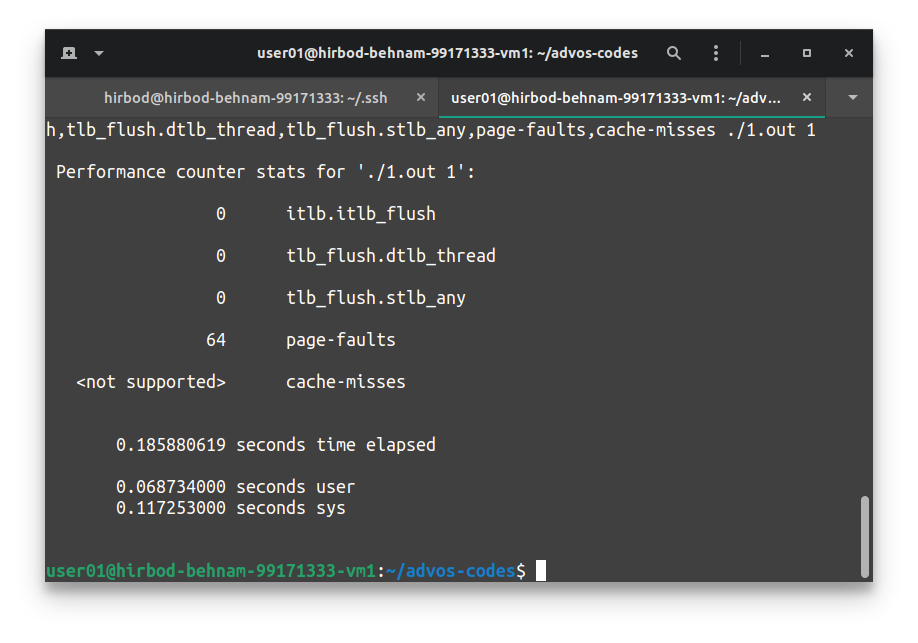
\includegraphics[scale=0.4]{pic/1-no-tlb.png}
    \caption{خروجی‌های 0 در فیلد‌های مربوط به \lr{TLB}}
\end{figure}
به صورت عجیبی تمامی مولفه‌های مربوط به
\lr{TLB}
برابر 0 بودند. اگر این مولفه‌ها مثل
\lr{cache-misses}
برابر
\lr{not supported}
بودند حداقل می‌دانستم که احتمالا ماشین‌های مجازی از این مورد پشتیبانی نمی‌کنند ولی این عدد برابر 0 است!
برای جست و جو بیشتر من یک ماشین مجازی
\lr{Debian 11}
را بر روی کامپیوتر خودم با مجازی سازی
\lr{VirtualBox}
اجرا کردم که تست کنم که آیا
\lr{VMWare} با \lr{VirtualBox}
فرقی دارد یا خیر. اما به صورت عجیبی در ماشین مجازی خودم اصلا
\lr{perf}
هیچ کدام از پارامتر‌های
\lr{TLB}
را نشناخت و برنامه به کل اجرا نشد! سپس از
\codeword{perf list}
استفاده کردم که بررسی کنم که آیا جایگزینی وجود دارد یا خیر که با
\codeword{tlb:tlb\_flush}
مواجه شدم. این پارامتر اصلا در
\codeword{perf list}
خود من و ماشین مجازی دانشکده وجود ندارد! ولی عجیب‌تر از آن اینکه این پارامتر بر روی تمامی دستگاه‌های من
(حتی با توجه به عدم وجود آن در \codeword{perf list})
کار می‌کند! 
\begin{figure}[H]
    \centering
    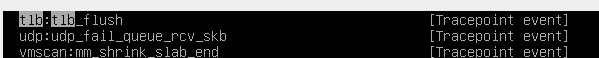
\includegraphics[scale=0.7]{pic/1-tlb-debian.png}
    \caption{نتیجه‌ی سرچ عبارت \lr{TLB} در \codeword{perf list} در \lr{debian}}
\end{figure}
همچنین من متوجه شدم که نمی‌توان از آرگومان‌هایی مثل
\codeword{dtlb\_load\_misses.miss\_causes\_a\_walk}
نیز برای تشخیص دادن تعداد
\lr{tlb miss}ها
در ماشین مجازی استفاده کرد. من تمامی آرگومان‌های مربوط به
\lr{DTLB miss}
را تست کردم ولی تمامی آن‌ها مقدار
0
را بر می‌گرداندند مانند شکل
\ref{fig:no_tlb_miss}.
\begin{figure}[H]
    \centering
    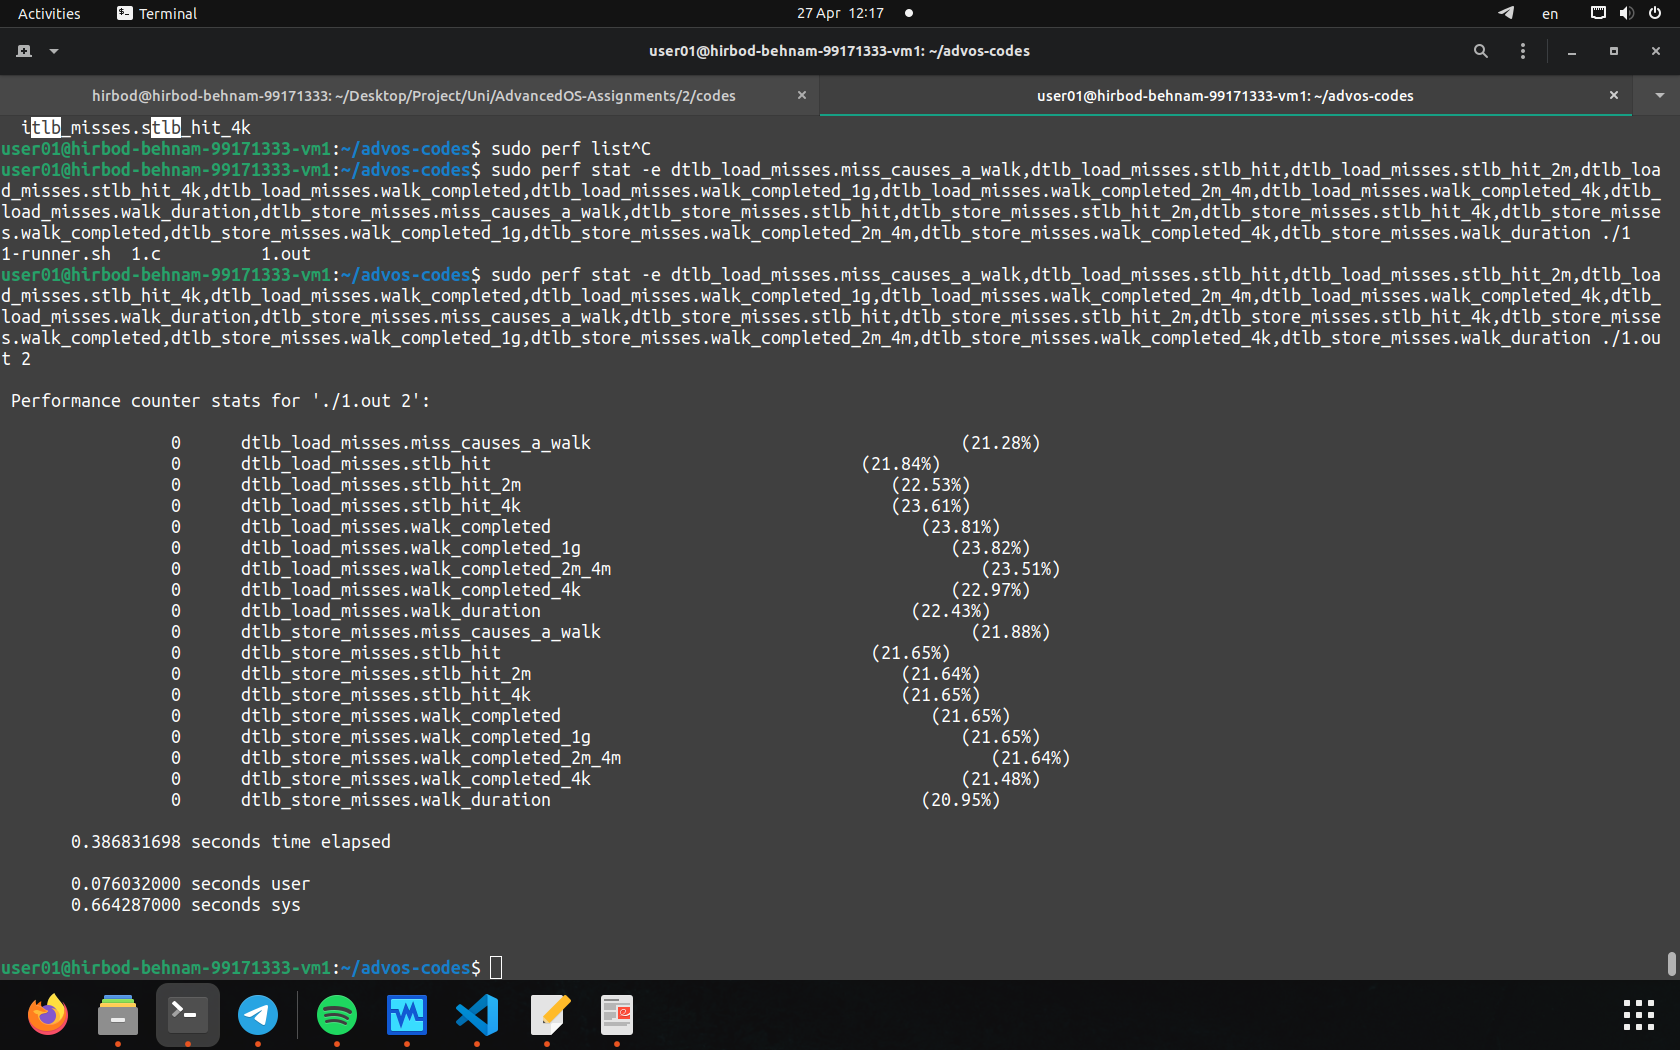
\includegraphics[scale=0.25]{pic/1-tlb-miss-vm.png}
    \caption{صفر بودن تمامی آرگومان‌های مربوط به \lr{TLB miss} در ماشین مجازی}
    \label{fig:no_tlb_miss}
\end{figure}

حال به کمک آرگومان
\codeword{tlb:tlb\_flush}
در ابتدا آزمایش را دوباره بر روی کامپیوتر شخصی خودم
انجام می‌دهم و سپس آنرا بر روی سرور‌های دانشگاه اجرا می‌کنیم.
نتایج بدست آمده به صورت
\lr{CSV}
در پوشه‌ی
\lr{codes}
موجود است. به صورت خلاصه نیز نتابج به صورت زیر هستند:
\begin{figure}[H]
    \centering
    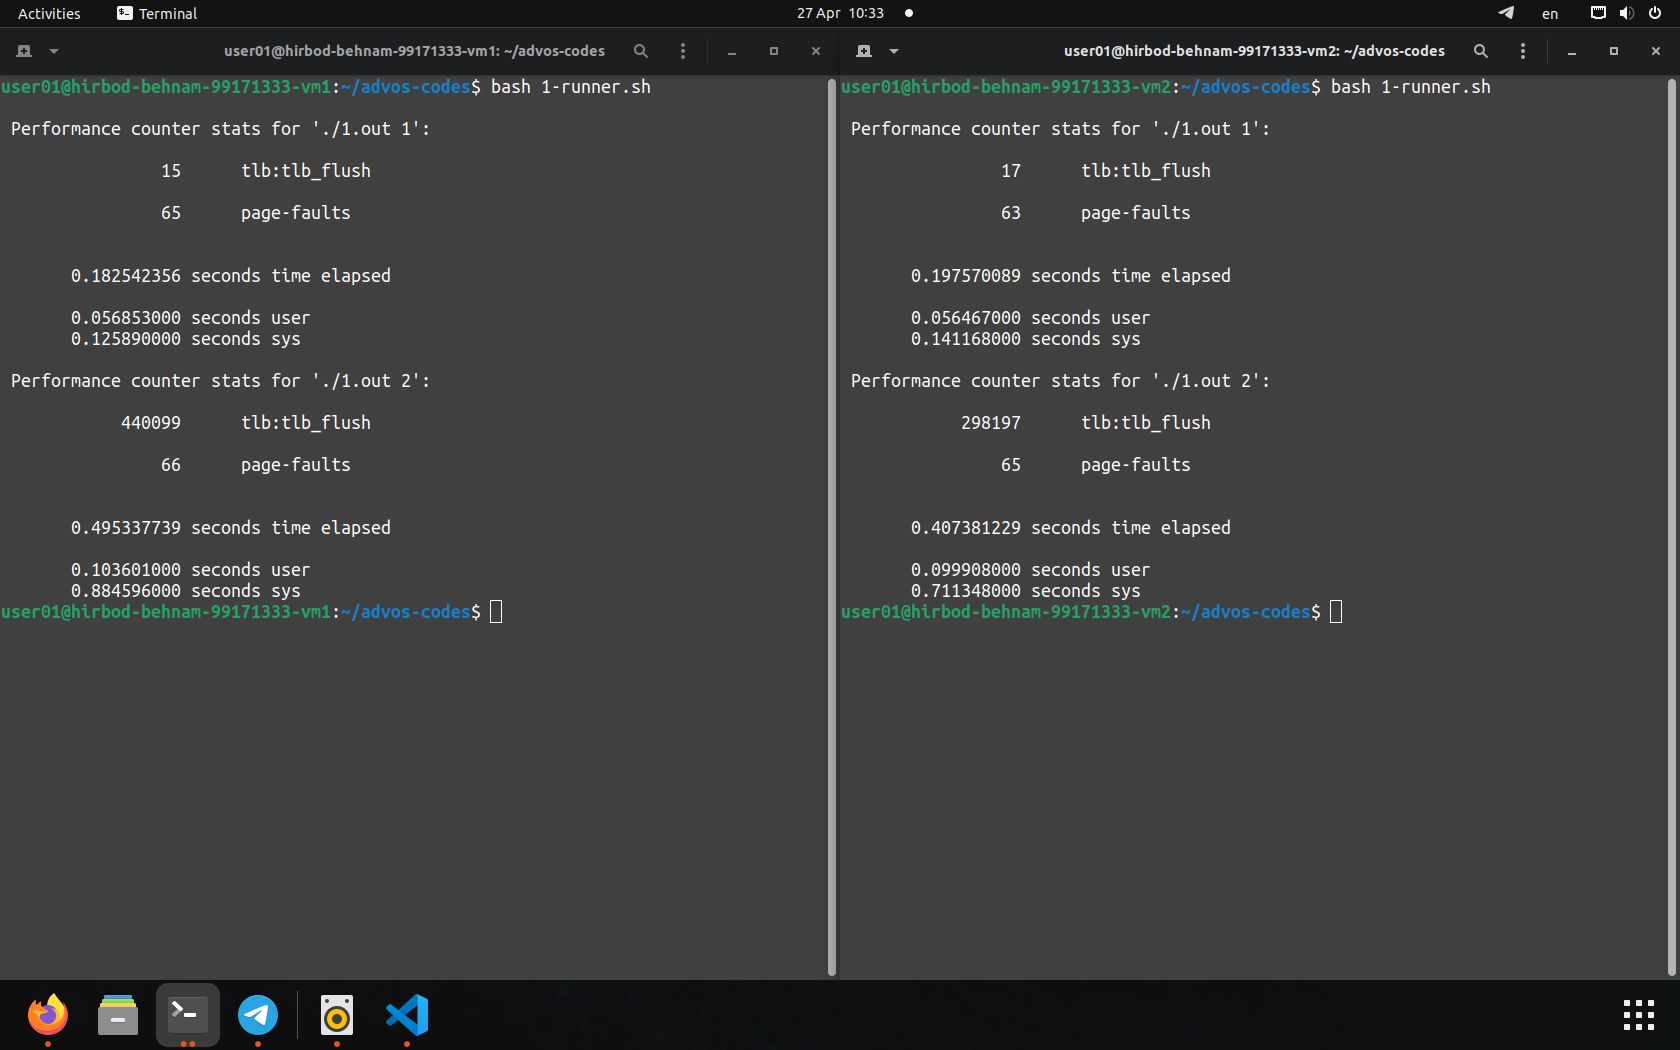
\includegraphics[scale=0.25]{pic/1-vm.png}
    \caption{ران کردن کد‌ها به صورت همزمان در ماشین‌های مجازی}
\end{figure}
\begin{figure}[H]
\small
\centering
\begin{latin}
\begin{tabular}{|c|ccc|ccc|}
    \hline
    \multirow{2}{*}{Thread Count} & \multicolumn{3}{|c|}{VM1} & \multicolumn{3}{|c|}{VM2}\\
    & TLB & Page Fault & Time & TLB & Page Fault & Time\\
    \hline
    1 & 15&65&0.182542356 & 17&63&0.197570089\\
    2 & 440099&66&0.495337739 & 298197&65&0.407381229\\
    3 & \multicolumn{3}{|c|}{-} & \multicolumn{3}{|c|}{-}\\
    4 & \multicolumn{3}{|c|}{-} & \multicolumn{3}{|c|}{-}\\
    5 & \multicolumn{3}{|c|}{-} & \multicolumn{3}{|c|}{-}\\
    6 & \multicolumn{3}{|c|}{-} & \multicolumn{3}{|c|}{-}\\
    7 & \multicolumn{3}{|c|}{-} & \multicolumn{3}{|c|}{-}\\
    \hline
\end{tabular}
\begin{tabular}{|c|cccc|}
    \hline
    \multirow{2}{*}{Thread Count} & \multicolumn{4}{|c|}{PC}\\
    & TLB Flush & TLB Miss & Page Fault & Time\\
    \hline
    1&15&101741&65&0.057957149\\
    2&158775&1730285&67&0.087978371\\
    3&963597&7518891&68&0.195919141\\
    4&1727973&13826423&69&0.251293690\\
    5&2277926&19421560&74&0.314809996\\
    6&3595825&26156164&75&0.418881412\\
    7&4981246&34637254&76&0.458051787\\
    \hline
\end{tabular}
\end{latin}
\caption{مشخصات اجرای بر روی هر یک از ماشین‌ها}
\end{figure}
حال سعی می‌کنیم که اعداد را تحلیل کنیم. در ابتدا متوجه می‌شویم که برنامه در ماشین‌های مجازی بیشتر از
یک ماشین واقعی طول کشیده است. این موضوع چندین دلیل می‌تواند داشته باشد. اولین دلیل اینکه مجازی سازی کند
است و
\lr{context switch}
برنامه می‌تواند بسیار زمان بر تر نسبت به یک ماشین بدون مجازی سازی باشد. همچنین دقت کنید که کلاک پردازنده‌ی
سرور‌های دانشگاه از کلاک پردازنده‌ی کامپیوتر من کمتر است. این موضوع نیز می‌تواند دلیلی بر کندتر
بودن برنامه باشد. یک نکته‌ی دیگر که می‌توان به آن اشاره کرد بیشتر طول کشیدن برنامه با تعداد ترد 2
بر روی ماشین مجازی اول نسبت به دومی است. این موضوع می‌تواند نشانگر این باشد که
\lr{TLB shootdown}های
ماشین مجازی دوم بر روی ماشین مجازی اول تاثیر گذاشته است و باعث شده است که برنامه‌ بر روی ماشین
مجازی اول مجبور شود که بیشتر \lr{page walk}
انجام دهند. همچنین می‌توان حدس زد که برنامه‌ بر روی ماشین مجازی دوم قبل از ماشین مجازی اول اجرا
شده است. این موضوع نیز درست است چرا که من اول برنامه بر روی ماشین مجازی دوم را اجرا کردم!

تعداد
\lr{page fault}ها
خیلی تفاوتی با حالت غیر مجازی هم ندارد و نمی‌توان نتیجه‌گیری خاصی از آن کرد. نتیجه‌گیری‌های تمرین قبلی
به نظر من برای این مورد نیز صادق است که آنرا اینجا نیز می‌آورم:
\begin{quote}
    نکته‌ای که چشم من را گرفت این است که
    \lr{page fault}
    با اینکه به صورت کاملا صعودی بالا رفته است،‌ ولی تعداد آن خیلی زیاد نیست. ما در هر ترد صد هزار بار
    \codeword{madvise}
    می‌کنیم. اما برای هر تردی که اضافه می‌شود تعداد 
    \lr{page fault}ها
    در حدود ۲ تا زیاد می‌شود. این رفتار به نظر من تقصیر
    \codeword{madvise}
    نیست. بلکه احتمالا تقصیر ساختن ترد‌ها و یا طول کشیدن بیشتر برنامه است. دقت کنید که مموری
    \lr{allocate}
    شده نیز برابر
    ۳۲ کیلوبایت یا
    ۸ صفحه است.
\end{quote}

در نهایت تعداد
\lr{TLB shootdown}ها
را بررسی می‌کنیم. در ابتدا چیزی که بر روی کامپیوتر خودم توجهم را جلب کرد پرش خیلی زیاد تعداد
\lr{shootdown}ها
زمانی است که تعداد ترد‌ها را من از 2 به 3 افزایش می‌دهم. این موضوع ممکن است که به خاطر
\lr{kernel thread}ها
باشد. احتمالا تنها
\lr{TLB}
مربوط به یک هسته‌ی مشخص از
\lr{CPU}
فلاش می‌شود و به خاطر اینکه نیازی نیست که بین هسته‌های دیگر پیامی جا به جا شود تعداد
\lr{TLB shootdown}ها
کمتر است. (چون که مثلا دیگر لازم نیست کاری با \lr{shared tlb} انجام دهیم.)

حال تعداد
\lr{TLB shootdown}ها
در
\lr{VM}
نسبت به ماشین واقعی را بررسی می‌کنیم. اولین چیزی که چشم ما را می‌گیرد این است که تعداد
\lr{shootdown}ها
بسیار بیشتر است. من برای تست فقط بر روی یک ماشین مجازی نیز تست کردم (یعنی همزمان برنامه‌ها را اجرا نکردم).
نتیجه به صورت زیر است:
\begin{figure}[H]
    \small
    \centering
    \begin{latin}
    \begin{tabular}{|c|ccc|}
        \hline
        \multirow{2}{*}{Thread Count} & \multicolumn{3}{|c|}{Single VM}\\
        & TLB & Page Fault & Time\\
        \hline
        1 & 17&63&0.152576567\\
        2 & 276551&66&0.349051301\\
        \hline
    \end{tabular}
    \end{latin}
    \caption{مشخصات اجرا بر روی یک ماشین مجازی}
\end{figure}
همان طور که مشاهده می‌شود هم سرعت برنامه بیشتر شد و هم تعداد
\lr{TLB shootdown}ها
کمتر شد. این موضوع نشانگر این است که وقتی دو ماشین مجازی با هم می‌خواهند که
\codeword{madvise}
را انجام دهند،‌ تاثیراتی را بر روی هم می‌گذارند که باعث می‌شود که هم کندتر شوند و هم اینکه
\lr{TLB shootdown}ها
بیشتر شود.

\smalltitle{آپدیت بعد از درست شدن مقادیر \lr{perf}:}
بعد از درست شدن مشکل
\lr{perf}
در
\lr{HPC}های
دانشگاه من باری دیگر همین تست‌ها را انجام دادم و نتیجه‌ی آنرا در زیر می‌آورم:
\begin{figure}[H]
    \small
    \centering
    \begin{latin}
    \begin{tabular}{|c|cccc|cccc|}
        \hline
        \multirow{2}{*}{Thread \#} & \multicolumn{4}{|c|}{VM1} & \multicolumn{4}{|c|}{VM2}\\
        & TLB Flush & TLB Miss & Page Fault & Time & TLB Flush & TLB Miss & Page Fault & Time\\
        \hline
        1 & 17&307884&67&0.194133870& 14&307371&65&0.196895015\\
        2 & 287663&4612810&64&0.403384311 & 300284&4578368&69&0.440842966\\
        \hline
    \end{tabular}
    \end{latin}
    \caption{مشخصات اجرای بر روی هر یک از ماشین‌ها}
\end{figure}
همان طور که مشاهده می‌شود تعداد
\lr{TLB flush} و \lr{page fault}
و سرعت اجرای برنامه که تغییری نکرده است. (مشخصا!)
اما متوجه می‌شویم که تعداد
\lr{TLB miss}ها
نسبت به حالت
\lr{bare metal}
تقریبا سه برابر شده است. این موضوع می‌تواند دو دلیل داشته باشد. یکی اینکه لود سرور زیاد است و دیگری
اینکه حجم
\lr{TLB}
سرور از
\lr{TLB}
من کمتر است. با توجه به
\link{https://www.cpu-world.com/CPUs/Xeon/Intel-Xeon\%20E5-2699\%20v4.html}{این لینک}
مشخصات
\lr{TLB}
پردازنده‌ی ماشین‌مجازی دانشگاه به صورت زیر است:
\begin{latin}
    \begin{itemize}
        \item 64-byte Prefetching
        \item Data TLB: 1-GB pages, 4-way set associative, 4 entries
        \item Data TLB: 4-KB Pages, 4-way set associative, 64 entries
        \item Instruction TLB: 4-KByte pages, 8-way set associative, 64 entries
        \item L2 TLB: 1-MB, 4-way set associative, 64-byte line size
        \item Shared 2nd-Level TLB: 4-KB / 2-MB pages, 6-way associative, 1536 entries. Plus, 1-GB pages, 4-way, 16 entries
    \end{itemize}
\end{latin}
و طبق
\link{https://www.cpu-world.com/CPUs/Core_i7/Intel-Core\%20i7-4790K.html}{این لینک}
مشخصات
\lr{CPU}
خودم را بررسی می‌کنم.
\begin{latin}
    \begin{itemize}
        \item 64-byte Prefetching
        \item Data TLB: 1-GB pages, 4-way set associative, 4 entries
        \item Data TLB: 4-KB Pages, 4-way set associative, 64 entries
        \item Instruction TLB: 4-KByte pages, 8-way set associative, 64 entries
        \item L2 TLB: 1-MB, 4-way set associative, 64-byte line size
        \item Shared 2nd-Level TLB: 4-KByte / 2-MB pages, 8-way associative, 1024 entries
    \end{itemize}
\end{latin}
نه تنها کمتر نیست بلکه تعداد
\lr{entry}های
\lr{shared TLB}
بیشتر نیز است! پس به احتمال زیاد دلیل اول است که باعث می‌شود تعداد
\lr{TLB miss}
ها زیاد شود مخصوصا وقتی که دو ماشین مجازی همزمان در حال استفاده از
\lr{TLB}
هستند.